% Created 2024-04-22 Δευ 12:18
% Intended LaTeX compiler: pdflatex
\documentclass[11pt]{report}
\usepackage[utf8]{inputenc}
\usepackage[T1]{fontenc}
\usepackage{graphicx}
\usepackage{longtable}
\usepackage{wrapfig}
\usepackage{rotating}
\usepackage[normalem]{ulem}
\usepackage{amsmath}
\usepackage{amssymb}
\usepackage{capt-of}
\usepackage{hyperref}
\usepackage{booktabs}
\usepackage{import}
\usepackage[LGR, T1]{fontenc}
\usepackage[greek, english, american]{babel}
\usepackage{alphabeta}
\usepackage{esint}
\usepackage{mathtools}
\usepackage{esdiff}
\usepackage{makeidx}
\usepackage{glossaries}
\usepackage{newfloat}
\usepackage{minted}
\usepackage{chemfig}
\usepackage{svg}
\usepackage{fancyhdr}
\usepackage[a4paper,width=150mm,top=25mm,bottom=25mm]{geometry}
\newcommand{\HRule}{\rule{\linewidth}{0.5mm}}
\date{}
\title{ΒΙΟΑΠΟΔΟΜΗΣΗ ΥΠΟΛΕΙΜΜΑΤΩΝ ΤΡΟΦΙΜΩΝ ΚΑΙ ΠΑΡΑΓΩΓΗ ΒΙΟΑΕΡΙΟΥ ΜΕΣΩ ΑΝΑΕΡΟΒΙΑΣ ΧΩΝΕΥΣΗΣ ΣΕ ΕΡΓΑΣΤΗΡΙΑΚΗ ΚΑΙ ΠΙΛΟΤΙΚΗ ΚΛΙΜΑΚΑ Draft της Εισαγωγής}
\hypersetup{
 pdfauthor={Βιδιάνος Γιαννίτσης},
 pdftitle={ΒΙΟΑΠΟΔΟΜΗΣΗ ΥΠΟΛΕΙΜΜΑΤΩΝ ΤΡΟΦΙΜΩΝ ΚΑΙ ΠΑΡΑΓΩΓΗ ΒΙΟΑΕΡΙΟΥ ΜΕΣΩ ΑΝΑΕΡΟΒΙΑΣ ΧΩΝΕΥΣΗΣ ΣΕ ΕΡΓΑΣΤΗΡΙΑΚΗ ΚΑΙ ΠΙΛΟΤΙΚΗ ΚΛΙΜΑΚΑ Draft της Εισαγωγής},
 pdfkeywords={},
 pdfsubject={},
 pdfcreator={Emacs 29.3 (Org mode 9.6.15)}, 
 pdflang={English}}
\makeatletter
\newcommand{\citeprocitem}[2]{\hyper@linkstart{cite}{citeproc_bib_item_#1}#2\hyper@linkend}
\makeatother

\usepackage[notquote]{hanging}
\begin{document}

\renewcommand{\abstractname}{Περίληψη}
\renewcommand{\tablename}{Πίνακας}
\renewcommand{\figurename}{Διάγραμμα}
\renewcommand{\chaptername}{Κεφάλαιο}
\renewcommand{\partname}{Μέρος}
\renewcommand{\listfigurename}{Περιεχόμενα Διαγραμμάτων: }
\renewcommand{\listtablename}{Περιεχόμενα Πινάκων: }
\renewcommand\listingscaption{Κώδικας}
\pagestyle{fancy}
\fancyhead{}
\fancyhead[L]{\chaptername~\thechapter}
\fancyhead[R]{Βιδιάνος Γιαννίτσης}

\renewcommand{\contentsname}{Κεφάλαια: }
\begin{titlepage}

\begin{center}
  \begin{minipage}{0.2\textwidth}
    \begin{flushleft}
      \includegraphics[width=1\textwidth]{~/Pictures/ntua_logo.png}\\[0.4cm]    
    \end{flushleft}
  \end{minipage}
  \begin{minipage}{0.75\textwidth}
    \textsc{\bfseries \Large ΕΘΝΙΚΟ ΜΕΤΣΟΒΙΟ ΠΟΛΥΤΕΧΝΕΙΟ}\\[0.2cm]
    \textsc{\bfseries \Large ΣΧΟΛΗ ΧΗΜΙΚΩΝ ΜΗΧΑΝΙΚΩΝ}\\[0.2cm]
    \textsc{\large \bfseries ΤΟΜΕΑΣ IV: ΣΥΝΘΕΣΗ ΚΑΙ ΑΝΑΠΤΥΞΗ ΒΙΟΜΗΧΑΝΙΚΩΝ ΔΙΑΔΙΚΑΣΙΩΝ}\\[0.2cm]
    \textsc{\bfseries \large ΕΡΓΑΣΤΗΡΙΟ ΟΡΓΑΝΙΚΗΣ ΧΗΜΙΚΗΣ \\ ΤΕΧΝΟΛΟΓΙΑΣ}\\[0.2cm]
  \end{minipage}
  \\[2.5cm]

  \HRule \\[0.3cm]
  \Huge Βιοαποδόμηση Υπολειμμάτων Τροφίμων και Παραγωγή Βιοαερίου μέσω Αναερόβιας Χώνευσης σε Εργαστηριακή και Πιλοτική Κλίμακα\\[2.5cm]

  \huge Διπλωματική Εργασία \\[0.3cm]
   \begin{minipage}{0.4\textwidth}
    \begin{flushleft}
      \emph{\LARGE Συγγραφέας:}\\
	\emph{\LARGE Αριθμός Μητρώου:} \\
	\emph{\LARGE e-mail:}
      \end{flushleft}
    \end{minipage}
    \begin{minipage}{0.4\textwidth}
      \begin{flushright} \large
	\LARGE Βιδιάνος Γιαννίτσης\\
	\LARGE ch19113\\
	\LARGE vidianosgiannitsis@gmail.com
      \end{flushright}
    \end{minipage}
    \HRule \\[0.3cm]
  \vfill
{\LARGE Αθήνα, 2024}

\end{center}

\end{titlepage}

\part*{Περιεχόμενα}
\label{sec:org477fd46}
\tableofcontents
\pagebreak

\listoffigures
\pagebreak

\listoftables

\part{Θεωρητικό Μέρος}
\label{sec:org0a64a05}
\chapter{Εισαγωγή}
\label{sec:org479bc92}
Τα υπολείμματα τροφών αποτελούν μία από τις σημαντικότερες κατηγορίες οργανικών αποβλήτων. Ο οργανισμός τροφίμων και αγρονομίας των ηνωμένων πολιτείων (FAO) υπολογίζει πως περίπου το 1/3 της παγκόσμιας παραγωγής τροφών (περίπου 1.3 δις τόνοι ετησίως) χάνεται κατά την παραγωγική διαδικασία ή απορρίπτεται. Κάποιες από αυτές τις απώλειες είναι αναπόφευχτες, αλλά πολλές θα μπορούσαν να αποφευχθούν ή τα υπολείμματα να συλλεχθούν για μία καλύτερη αξιοποίηση, καθώς οι κλασσικές τεχνικές, όπως η υγειονομική ταφή ή η αποτέφρωση, δημιουργούν προβλήματα όπως οι ανεξέλεγκτες εκπομπές μεγάλων ποσοτήτων αερίων του θερμοκηπίου (\citeprocitem{9}{Wu et al. 2022}; \citeprocitem{10}{Zhang et al. 2020}; \citeprocitem{2}{Ishangulyyev, Kim, and Lee 2019}).

Συγκεκριμένα, έχει προσδιοριστεί πως το ισοδύναμο διοξειδίου του άνθρακα που παράγεται λόγω της μη ορθής αυτής διαχείρισης των υπολείμματων ανέρχεται στους 3.3 δις τόνους (\citeprocitem{7}{Taheri et al. 2021}) . Ακόμη, έχει βρεθεί πως τα υπολείμματα τροφών που οφείλονται μόνο στην απόρριψη τροφών από καταναλωτές σε ανεπτυγμένες χώρες είναι σχεδόν όσα παράγουν οι υπό σακχάριες και αφρικανικές χώρες συνολικά (περίπου 230 εκατομμύρια). Οπότε η αποφυγή της δημιουργίας τόσων υπολειμμάτων - ή η καλύτερη αξιοποίηση τους - θα μπορούσε να λύσει πολλά προβλήματα υποσιτισμού. Ακόμη και στον οικονομικό τομέα, δημιουργούνται σοβαρά προβλήματα από την ανεξέλεγκτη αυτή απόρριψη καθώς η καθαρή αξία των τροφών που χάνονται ή απορρίπτονται σε κάποιο σημείο της εφοδιαστικής αλυσίδας είναι 936 δις δολλάρια ανά έτος με ελάχιστο κέρδος, καθώς πολύ μικρές ποσότητες των υπολειμμάτων αυτών αξιοποιούνται (\citeprocitem{2}{Ishangulyyev, Kim, and Lee 2019}) . Συμπερασματικά, η δημιουργία αυτών των υπέρογκων ποσοτήτων υπολειμμάτων τροφών πλήγει κάθε πυλώνα της βιωσιμότητας και είναι ένα πάρα πολύ σοβαρό πρόβλημα.

Μία από τις βασικότερες υποκατηγορίες υπολειμμάτων τροφών είναι τα οικιακά υπολείμματα τροφών. Αποτελούν το μεγαλύτερο κομμάτι της παγκόσμιας παραγωγής υπολειμμάτων τροφών, αποτελώντας περίπου το \(61 \%\) αυτής (\citeprocitem{5}{“Statista - The Statistics Portal” n.d.}) . Στο \figurename \ref{fig:org398c113} φαίνεται η παγκόσμια παραγωγή υπολειμμάτων τροφών ανά τομέα.
\begin{figure}[htbp]
\centering
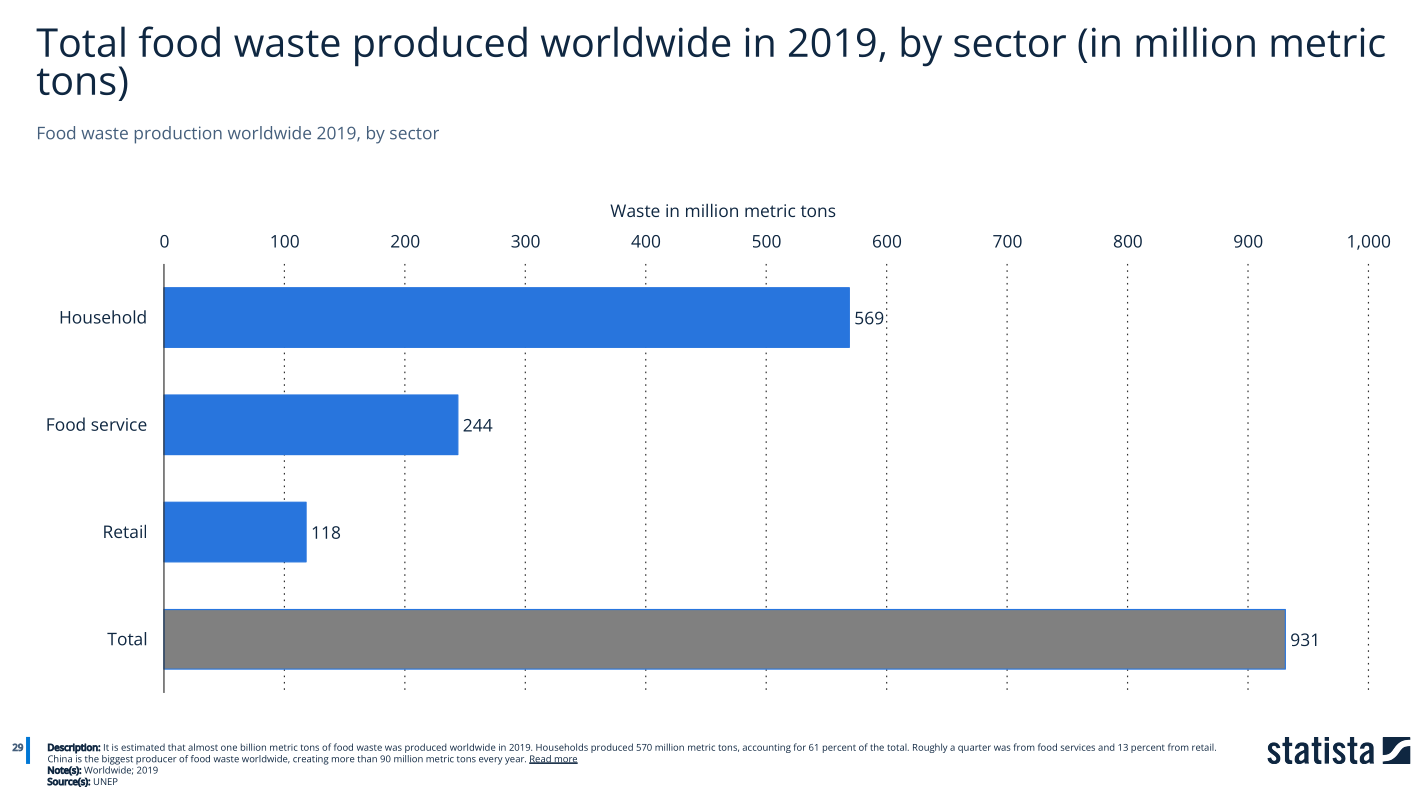
\includegraphics[width=.9\linewidth]{../plots/statistics/statistic_food_waste_by_sector_2019.png}
\caption{\label{fig:org398c113}Παγκόσμια παραγωγή υπολειμμάτων τροφών ανά τομέα}
\end{figure}

Η Ελλάδα είναι η χώρα με την δεύτερη μεγαλύτερη παραγωγή οικιακών υπολειμμάτων τροφών κατά κεφαλήν παγκοσμίως (142 κιλά/άτομο ετησίως) (\citeprocitem{5}{“Statista - The Statistics Portal” n.d.}) . Η παραγωγή υπολειμμάτων τροφών, ειδικά στον τομέα της κατανάλωσης, όπου βρίσκονται τα οικιακά υπολείμματα, καθώς και αυτά της εστίασης, είναι πολύ συχνά αναπόφευχτη. Οπότε, παρόλο που με πιο σωστές πρακτικές θα μπορούσαν να παράγονται λιγότερα υπολείμματα, η ανάπτυξη τεχνολογιών αξιοποίησης των υπολειμμάτων αυτών είναι πάρα πολύ σημαντικές. Οι τεχνολογίες αυτές θα πρέπει να είναι εύκολα εφαρμόσιμες και οικονομικές και η κλιμάκωση τους να είναι εφικτή.

Γενικά, η αγορά της διαχείρισης αποβλήτων είναι αρκετά μεγάλη (υπολογίζεται περίπου στα 1293 δις δολλάρια ετησίως από μία μελέτη του 2022), ενώ προβλέψεις λένε πως θα φτάσει τα 2000 δις μέχρι το 2030 και τα οργανικά απόβλητα, ως ένα πολύ σημαντικό ποσοστό των αστικών αποβλήτων (περίπου \(40-45 \%\)) είναι μία από τις βασικές περιοχές ενδιαφέροντος της αγοράς αυτής (\citeprocitem{5}{“Statista - The Statistics Portal” n.d.}) . Μία από τις βασικότερες τεχνολογίες που έχουν αναδειχθεί σε αυτήν την αγορά η οποία έχει δει ραγδαία αύξηση τα τελευταία χρόνια είναι η αναερόβια χώνευση. Η αναερόβια χώνευση χρησιμοποιεί οργανικά απόβλητα ως υπόστρωμα και με μία σειρά βιοχημικών διεργασιών, τα μετατρέπει σε πτητικά λιπαρά οξέα (VFAs) και τελικά μεθάνιο και διοξείδιο του άνθρακα (το μίγμα γνωστό ως βιοαέριο), το οποίο είναι ένας πολύ καλός ενεργειακός φορέας. Τα υπολείμματα τροφών είναι ένα πολύ καλό υπόστρωμα για αναερόβια χώνευση καθώς είναι πλούσια σε οργανικές ενώσεις αλλά και θρεπτικά στοιχεία και μπορούν να μετατραπούν πολύ αποτελεσματικά σε βιοαέριο. Στο \figurename \ref{fig:org7c75a94} φαίνεται η παγκόσμια παραγωγή ενέργειας από βιοαέριο τα τελευταία 15 χρόνια (\citeprocitem{5}{“Statista - The Statistics Portal” n.d.}) .

\begin{figure}[htbp]
\centering
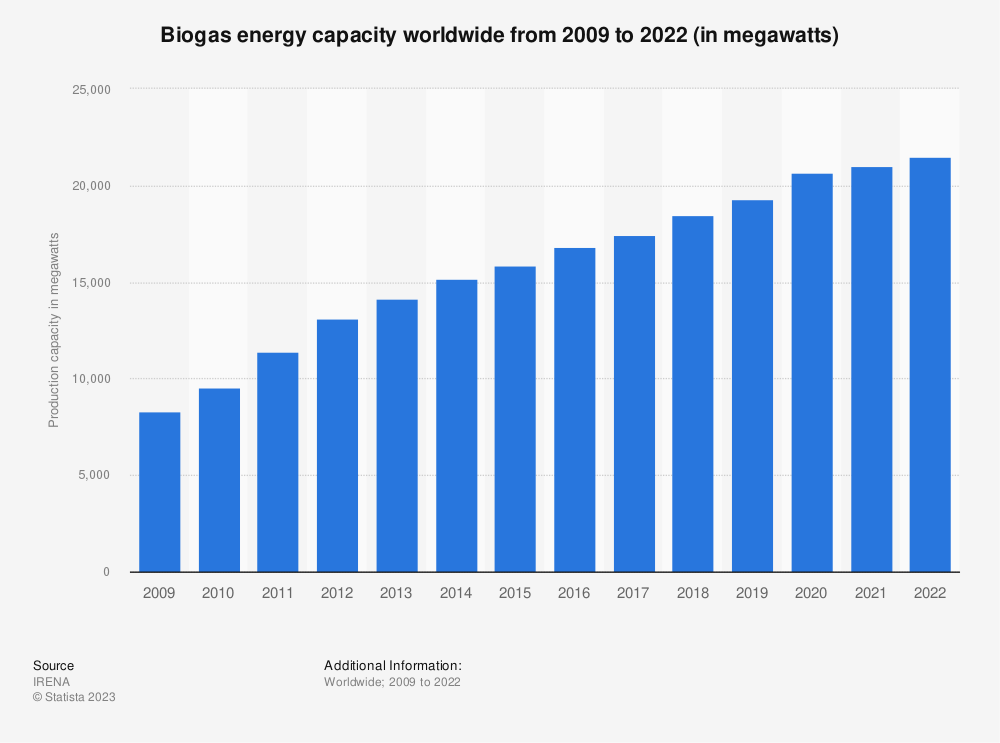
\includegraphics[width=.9\linewidth]{../plots/statistics/statistic_id1032922_global-biogas-energy-capacity-2009-2022.png}
\caption{\label{fig:org7c75a94}Παγκόσμια παραγωγή ενέργειας από βιοαέριο}
\end{figure}

Εκτός όμως από την αξιοποίηση του μεγάλου βιοχημικού δυναμικού των υπολειμμάτων αυτών, η αναερόβια χώνευση λύνει και άλλο ένα από τα σημαντικά προβλήματα του 21ου αιώνα, το οποίο είναι η ενέργεια. Αυτή τη στιγμή, πάνω από το \(80 \%\) της ενέργειας που καταναλώνεται παγκοσμίως βασίζεται σε μη ανανεώσιμες πηγές όπως το πετρέλαιο και το φυσικό αέριο. Οι ενεργειακές απαιτήσεις παγκοσμίως έχουν μία συνεχή αύξηση, ενώ οι πρώτες ύλες αυτές εξαλείφονται (\citeprocitem{5}{“Statista - The Statistics Portal” n.d.}) . Οπότε, τεχνολογίες παραγωγής ενέργειας από ανανεώσιμες πηγές, οι οποίες να έχουν το δυναμικό να αντικαταστήσουν τις πηγές αυτές θα γίνουν απαραίτητες τα επόμενα χρόνια. Οι περισσότερες τεχνολογίες ανανεώσιμης ενέργειας (πχ αιολική, ηλιακή ή υδροηλεκτρική ενέργεια) έχουν δυσκολία να φτάσουν τέτοια επίπεδα και για αυτό χρησιμοποιούνται επικουρικά σε μία κύρια πηγή ενέργειας (αυτή τη στιγμή, περίπου το \(30 \%\) της παγκόσμιας παραγωγής ηλεκτρισμού οφείλεται σε τέτοιες πηγές) (\citeprocitem{5}{“Statista - The Statistics Portal” n.d.}) . Τα υπολείμματα τροφών από την άλλη είναι άφθονα οπότε θεωρείται πως μία αποτελεσματική επεξεργασία θα μπορέσουν να καλύψουν ένα πολύ σημαντικό ποσοστό της παγκόσμιας ανάγκης σε ενέργεια.

Σκοπός της παρούσας μελέτης είναι η ανάπτυξη μίας μεθόδου επεξεργασίας των υπολειμμάτων τροφίμων, αρχικά, μέσω της βιοαποδόμησής τους με χρήση σκευασμάτων ενζύμων και μικροοργανισμών του εμπορίου, και στη συνέχεια, μέσω αναερόβιας χώνευσης για την παραγωγή βιοαερίου, η οποία θα αξιολογηθεί σε εργαστηριακή αλλά και πιλοτική κλίμακα.

\section{Υδρόλυση}
\label{sec:org77c64ed}
Η υδρόλυση γίνεται γενικά με 3 βασικές τεχνολογίες. Η πρώτη, είναι η θερμική υδρόλυση. Βασίζεται στην αύξηση της θερμοκρασίας, ώστε να αποικοδομηθούν τα πολυμερή και να είναι πιο εύκολη η αξιοποιήση του υπολείμματος. Ενδείκνειται για δύσκολα αποδομήσιμη βιομάζα, όπου είναι δύσκολο να χρησιμοποιηθεί κάποια άλλη τέχνικη. Βέβαια, λόγω των πολύ υψηλών ενεργειακών απαιτήσεων τους, δεν είναι ιδιαίτερα ελκυστικές για τα υπολείμματα τροφών, τα οποία είναι σχετικά εύκολα αποδομήσιμα (\citeprocitem{4}{Ma et al. 2018}).

Μία άλλη τεχνολογία είναι η χημική υδρόλυση. Βασίζεται στην χρήση κάποιων χημικών με ακραίες τιμές pH (είτε ισχυρά όξινα ή αλκαλικά), τα οποία μπορούν να προκαλέσουν κατάρρευση της πολυμερικής δομής και να απελευθερώσουν μικρότερα μόρια. Είναι μία πολύ φθηνή μέθοδος η οποία είναι όμως αποτελεσματική και για αυτό έχει ευρεία εφαρμογή. Όμως, στο περιβάλλον αυτό μπορούν να γίνουν ανεπιθύμητες αντιδράσεις, των οποίων τα προιόντα δρουν παρεμποδιστικά στις περισσότερες βιολογικές διεργασίες. Οπότε, παρόλο που η υδρόλυση θα έχει καλή απόδοση, το επόμενο στάδιο, που είναι και το στάδιο της αξιοποιήσης του υπολείμματος, δεν θα είναι πολύ αποδοτικό (\citeprocitem{4}{Ma et al. 2018}; \citeprocitem{1}{Han et al. 2016}) .

Η τρίτη τεχνολογία είναι η ενζυμική υδρόλυση. Σε αυτήν, ειδικά ένζυμα, όπως οι υδατανθρακάσες, οι πρωτεάσες και οι κυτταρινάσες διασπούν τα πολυμερή σε μικρότερα μόρια. Δεν έχουν παραπροιόντα, χρησιμοποιούν ήπιες συνθήκες και έχουν την καλύτερη απόδοση από τις 3 τεχνολογίες (\citeprocitem{1}{Han et al. 2016}; \citeprocitem{4}{Ma et al. 2018}) . Παρότι έχουν αυτά τα πλεονεκτήματα, έχουν ένα πολύ σημαντικό μειωνέκτημα. Το κόστος ενός ενζυμικού σκευάσματος για να γίνει σε μεγάλη κλίμακα η υδρόλυση είναι πολύ υψηλό, το οποίο εμποδίζει την εφαρμογή της τεχνολογίας αυτής. Βέβαια, μία αναλυτική οικονομική ανάλυση, η οποία σύγκρινε την ενζυμική με την χημική υδρόλυση, έδειξε πως ακόμη και με το αυξημένο κόστος της ενζυμικής υδρόλυσης, έχει μεγαλύτερο κέρδος λόγω της πολύ αυξημένης απόδοσης της συγκριτικά με την χημική υδρόλυση (\citeprocitem{10}{Zhang et al. 2020}) .

\section{Ενζυμική Υδρόλυση}
\label{sec:org8428ad7}
Καθώς η ενζυμική υδρόλυση θεωρείται η καλύτερη τεχνική για την βιοαποδόμηση των υπολειμμάτων τροφών, αλλά έχει το πρόβλημα του αρκετά αυξημένου κόστους, υπάρχει αρκετή μελέτη προσανατολισμένη στην μείωση του κόστους της ενζυμικής υδρόλυσης. Μία ιδέα που έχει προταθεί είναι η χρήση υπερήχων ως επικουρική προεπεξεργασία. Οι υπέρηχοι δημιουργούν ελεύθερες ρίζες υδροξυλίου οι οποίες είναι αντιδραστικές και μπορούν να συνεισφέρουν στην διάσπαση των πολυμερών (\citeprocitem{8}{Usmani et al. 2021}; \citeprocitem{6}{Suresh et al. 2020}; \citeprocitem{4}{Ma et al. 2018}) . Μία πιο αναλυτική μελέτη έδειξε πως σε batch πειράματα, η προεπεξεργασία με υπερήχους οδήγησε σε \(10 \%\) καλύτερη αποδοτικότητα και σε μείωση του απαραίτητου χρόνου επεξεργασίας στο μισό. Σε ένα συνεχές σύστημα, αυτό θα σήμαινε μείωση της απαραίτητης ποσότητας ένζυμων στο μισό, το οποίο είναι μία πολύ σημαντική βελτίωση (\citeprocitem{3}{Li et al. 2019}) . Όμως, η χρήση των υπερήχων έχει και αυτή ένα κόστος, το οποίο ειδικά σε μεγάλη κλίμακα είναι υψηλό. Οπότε, παρόλο που η τεχνολογία αυτή αυξάνει την απόδοση και μειώνει το κόστος, αυτό παραμένει αρκετά υψηλό, οπότε δεν μπορεί να θεωρηθεί μία τεχνική που θα επιτρέψει στην φθηνή μαζική επεξεργασία των υπολειμμάτων.

\textbf{πιθανόν να προσθέσω και κάποια άλλη παρόμοια προσπάθεια αν βρω}

Μία υποσχόμενη και οικονομικά εφαρμόσιμη λύση για το πρόβλημα αυτό είναι η χρήση σκευασμάτων τα οποία περιέχουν ένζυμα και μικροοργανισμούς. Το κόστος ενός τέτοιου σκευάσματος είναι σημαντικά χαμηλότερο από κάποιο το οποίο έχει μόνο ένζυμα, όμως, μπορεί να κάνει και αυτό αποτελεσματική βιοαποδόμηση. Ταυτόχρονα με την υδρόλυση, γίνεται και μία ζύμωση των υπολειμμάτων, η οποία παράγει προιόντα όπως η αιθανόλη και πτητικά λιπαρά οξέα (VFAs) όπως το οξικό, το προπιονικό και το γαλακτικό. Η ζύμωση αυτή κατατάσσεται στην κατηγορία οξεογενετικής ζύμωσης μικτής καλλιέργειας, η οποία είναι αρκετά μελετημένη στην βιβλιογραφία (σίγουρα χρειάζεται κάποια citations αλλά θα πρέπει να τα οργανώσω λίγο).

\section{Σκευάσματα με ένζυμα και μικροοργανισμούς}
\label{sec:orgd713812}
Τα προιόντα αυτής της μικτής διεργασίας είναι προιόντα τα οποία έχουν σημαντική αξία, οπότε μία τεχνολογία αξιοποίησης θα μπορούσε να είναι και η απευθείας ανάκτηση τους. Εναλλακτικά, μπορούν αυτά να χρησιμοποιηθούν ως ένα πιο κατάλληλο υπόστρωμα - σε σχέση με τα υπολείμματα τροφών - για κάποια άλλη διεργασία, όπως η αναερόβια χώνευση. Τα αρχικά στάδια της αναερόβιας χώνευσης είναι άλλωστε η υδρόλυση και η οξεογένεση, οπότε η διεξαγωγή τους σε ξεχωριστό αντιδραστήρα δεν δημιουργεί πρόβλημα. Μάλιστα, σε κάποιες περιπτώσεις είναι και πιο επιθυμητή η διεξαγωγή της αναερόβιας χώνευσης σε πολλά στάδια καθώς επιτρέπει καλύτερο έλεγχο της διεργασίας και συχνά αποφέρει καλύτερη απόδοση από ότι να γίνουν όλα σε ένα στάδιο (και για αυτό έχω κάποια citations).

Βέβαια, είτε στην περίπτωση ανάκτησης των προιόντων αυτών ή της χρήσης τους σε κάποια άλλη διεργασία, είναι πολύ σημαντικό, να κατανοηθεί ο μηχανισμός της ζύμωσης αυτής και ποιές αντιδράσουν συμβαίνουν, ώστε να μπορέσει μετά να ελεγχθεί η ζύμωση προς τα πιο επιθυμητά προιόντα ανά την εφαρμογή.

\section{Αναερόβια Χώνευση}
\label{sec:orga58c656}

\part*{Βιβλιογραφία}
\label{sec:orge9a96bf}
\begin{hangparas}{1.5em}{1}
\hypertarget{citeproc_bib_item_1}{Han, Wei, Yingting Yan, Yiwen Shi, Jingjing Gu, Junhong Tang, and Hongting Zhao. 2016. “Biohydrogen Production from Enzymatic Hydrolysis of Food Waste in Batch and Continuous Systems.” \textit{Scientific Reports} 6 (1): 38395. \url{https://doi.org/10.1038/srep38395}.}

\hypertarget{citeproc_bib_item_2}{Ishangulyyev, Rovshen, Sanghyo Kim, and Sang Hyeon Lee. 2019. “Understanding Food Loss and Waste–-Why Are We Losing and Wasting Food?” \textit{Foods} 8 (8): 297. \url{https://doi.org/10.3390/foods8080297}.}

\hypertarget{citeproc_bib_item_3}{Li, X., S. Mettu, G.J.O. Martin, M. Ashokkumar, and C.S.K. Lin. 2019. “Ultrasonic Pretreatment of Food Waste to Accelerate Enzymatic Hydrolysis for Glucose Production.” \textit{Ultrasonics Sonochemistry} 53: 77–82. \url{https://doi.org/10.1016/j.ultsonch.2018.12.035}.}

\hypertarget{citeproc_bib_item_4}{Ma, Chaonan, Jianyong Liu, Min Ye, Lianpei Zou, Guangren Qian, and Yu-You Li. 2018. “Towards Utmost Bioenergy Conversion Efficiency of Food Waste: Pretreatment, Co-Digestion, and Reactor Type.” \textit{Renewable and Sustainable Energy Reviews} 90 (July): 700–709. \url{https://doi.org/10.1016/j.rser.2018.03.110}.}

\hypertarget{citeproc_bib_item_5}{“Statista - The Statistics Portal.” n.d. https://www.statista.com/. Accessed November 13, 2023.}

\hypertarget{citeproc_bib_item_6}{Suresh, T., N. Sivarajasekar, K. Balasubramani, Tansir Ahamad, Manawwer Alam, and Mu Naushad. 2020. “Process Intensification and Comparison of Bioethanol Production from Food Industry Waste (Potatoes) by Ultrasonic Assisted Acid Hydrolysis and Enzymatic Hydrolysis: Statistical Modelling and Optimization.” \textit{Biomass and Bioenergy} 142 (November): 105752. \url{https://doi.org/10.1016/j.biombioe.2020.105752}.}

\hypertarget{citeproc_bib_item_7}{Taheri, Mir Edris, Erfaneh Salimi, Konstantinos Saragas, Jelica Novakovic, Elli Maria Barampouti, Sofia Mai, Dimitris Malamis, Konstantinos Moustakas, and Maria Loizidou. 2021. “Effect of Pretreatment Techniques on Enzymatic Hydrolysis of Food Waste.” \textit{Biomass Conversion and Biorefinery} 11 (2): 219–26. \url{https://doi.org/10.1007/s13399-020-00729-7}.}

\hypertarget{citeproc_bib_item_8}{Usmani, Zeba, Minaxi Sharma, Abhishek Kumar Awasthi, Gauri Dutt Sharma, Denise Cysneiros, S. Chandra Nayak, Vijay Kumar Thakur, Ravi Naidu, Ashok Pandey, and Vijai Kumar Gupta. 2021. “Minimizing Hazardous Impact of Food Waste in a Circular Economy – Advances in Resource Recovery through Green Strategies.” \textit{Journal of Hazardous Materials} 416 (August): 126154. \url{https://doi.org/10.1016/j.jhazmat.2021.126154}.}

\hypertarget{citeproc_bib_item_9}{Wu, Lan, Wei Wei, Xuran Liu, Dongbo Wang, and Bing-Jie Ni. 2022. “Potentiality of Recovering Bioresource from Food Waste through Multi-Stage Co-digestion with Enzymatic Pretreatment.” \textit{Journal of Environmental Management} 319 (October): 115777. \url{https://doi.org/10.1016/j.jenvman.2022.115777}.}

\hypertarget{citeproc_bib_item_10}{Zhang, Cunsheng, Xinxin Kang, Fenghuan Wang, Yufei Tian, Tao Liu, Yanyan Su, Tingting Qian, and Yifeng Zhang. 2020. “Valorization of Food Waste for Cost-Effective Reducing Sugar Recovery in a Two-Stage Enzymatic Hydrolysis Platform.” \textit{Energy} 208 (October): 118379. \url{https://doi.org/10.1016/j.energy.2020.118379}.}\bigskip
\end{hangparas}
\end{document}
